%==============================================================================
%  STAT 5200 - Applied Econometrics I
%  Homework 2
%
%  Compile with:  pdflatex "HW 2 - Report.tex"  (run twice for refs)
%
%  Directory layout assumed by this file:
%     HW 2 - Report.tex
%     R/        (scripts, for Q5)
%     figures/  (generated figures, for Q5)
%     output/   (captured console output, for Q5)
%==============================================================================
\documentclass[11pt]{article}

\usepackage[margin=1in]{geometry}
\usepackage[T1]{fontenc}
\usepackage[utf8]{inputenc}
\usepackage{amsmath,amssymb}
\usepackage{booktabs}
\usepackage{graphicx}
\usepackage{xcolor}
\usepackage{listings}
\usepackage[font=small,labelfont=bf]{caption}
\usepackage[hidelinks]{hyperref}

%------------------------------------------------------------------------------
%  Code presentation (used from Q5 onwards)
%
%  Code is set as selectable text on a fixed character grid, source and console
%  output are given visually distinct styles, and source lines are kept to 76
%  characters so that nothing wraps.
%------------------------------------------------------------------------------
\definecolor{codekeyword}{RGB}{0,86,148}
\definecolor{codestring} {RGB}{163,21,21}
\definecolor{codecomment}{RGB}{106,115,125}
\definecolor{codebg}     {RGB}{248,248,250}
\definecolor{coderule}   {RGB}{220,220,226}

\lstdefinestyle{Rcode}{
  language        = R,
  basicstyle      = \ttfamily\footnotesize,
  keywordstyle    = \color{codekeyword}\bfseries,
  stringstyle     = \color{codestring},
  commentstyle    = \color{codecomment}\itshape,
  numbers         = left,
  numberstyle     = \ttfamily\scriptsize\color{codecomment},
  numbersep       = 9pt,
  backgroundcolor = \color{codebg},
  frame           = single,
  rulecolor       = \color{coderule},
  framesep        = 4pt,
  xleftmargin     = 15pt,
  xrightmargin    = 0pt,
  columns         = fixed,
  basewidth       = 0.5em,
  keepspaces      = true,
  tabsize         = 2,
  showstringspaces = false,
  breaklines      = true,
  breakatwhitespace = true,
  postbreak       = \mbox{\textcolor{codekeyword}{$\hookrightarrow$}\space},
  captionpos      = b,
  abovecaptionskip = 6pt,
}

\lstdefinestyle{Routput}{
  language        = {},
  basicstyle      = \ttfamily\footnotesize,
  keywordstyle    = \ttfamily,
  commentstyle    = \ttfamily,
  stringstyle     = \ttfamily,
  numbers         = none,
  backgroundcolor = \color{white},
  frame           = leftline,
  rulecolor       = \color{coderule},
  framesep        = 6pt,
  xleftmargin     = 20pt,
  breaklines      = true,
  captionpos      = b,
  abovecaptionskip = 6pt,
}

\lstset{style=Rcode}
\renewcommand{\lstlistingname}{Listing}

% Short inline code fragments.
\newcommand{\code}[1]{\texttt{#1}}

% Operators used throughout.
\DeclareMathOperator{\Var}{Var}
\DeclareMathOperator{\Cov}{Cov}
\DeclareMathOperator{\Avar}{Avar}
\DeclareMathOperator{\sd}{sd}

%------------------------------------------------------------------------------
\title{\vspace{-2em}Homework 2\\[0.3em]
       \large STAT 5200 --- Applied Econometrics I --- Fall 2026}

\author{Apostolos Kyratzis - 13130833}
\date{October 1, 2026}

\begin{document}
\maketitle

%==============================================================================
\section{Q1: Reflection}
%==============================================================================

\emph{To be completed.}

%==============================================================================
\section{Q2: Conditional expectation}
\label{sec:q2}
%==============================================================================

Throughout, $w = (y,x)'$ is normally distributed with mean $\mu = (\mu_y,
\mu_x)'$ and covariance matrix
\[
\Sigma =
\begin{pmatrix}
\sigma_y^2 & \sigma_y\sigma_x\rho\\
\sigma_x\sigma_y\rho & \sigma_x^2
\end{pmatrix},
\qquad
|\Sigma| = \sigma_y^2\sigma_x^2(1-\rho^2).
\]
It is convenient to write the standardised variables
\[
z_y = \frac{y-\mu_y}{\sigma_y},
\qquad
z_x = \frac{x-\mu_x}{\sigma_x},
\]
so that the joint and marginal densities supplied in the question read
\[
f_{Y,X}(y,x) = \frac{1}{2\pi\sigma_y\sigma_x(1-\rho^2)^{1/2}}
  \exp\!\left(-\frac{1}{2(1-\rho^2)}
  \left[z_y^2 - 2\rho z_y z_x + z_x^2\right]\right),
\]
\[
f_X(x) = \frac{1}{\sqrt{2\pi}\,\sigma_x}
  \exp\!\left(-\tfrac{1}{2}z_x^2\right).
\]

\paragraph{(1) The conditional distribution of $y$ given $x$.}
By definition $f_{Y|X}(y|x) = f_{Y,X}(y,x)/f_X(x)$. The constants divide to
\[
\frac{1}{2\pi\sigma_y\sigma_x(1-\rho^2)^{1/2}}
\Bigg/ \frac{1}{\sqrt{2\pi}\,\sigma_x}
= \frac{1}{\sqrt{2\pi}\,\sigma_y(1-\rho^2)^{1/2}},
\]
so that $\sigma_x$ cancels and only $\sigma_y$ and $\rho$ survive. The two
exponents combine into
\[
-\frac{1}{2(1-\rho^2)}\left[z_y^2 - 2\rho z_y z_x + z_x^2\right]
+ \frac{1}{2}z_x^2
= -\frac{1}{2(1-\rho^2)}
  \left[z_y^2 - 2\rho z_y z_x + z_x^2 - (1-\rho^2)z_x^2\right],
\]
where the second term has been taken inside the bracket by multiplying it by
$-(1-\rho^2)/(1-\rho^2)$. Since $z_x^2 - (1-\rho^2)z_x^2 = \rho^2 z_x^2$, the
bracket is a perfect square:
\[
z_y^2 - 2\rho z_y z_x + \rho^2 z_x^2 = \left(z_y - \rho z_x\right)^2 .
\]
This is the step that the completion of the square in Notes 01 performs. It
remains to express it in the original units. Factoring $1/\sigma_y$ out of
\[
z_y - \rho z_x
= \frac{y-\mu_y}{\sigma_y} - \rho\,\frac{x-\mu_x}{\sigma_x}
= \frac{1}{\sigma_y}
  \left[y - \mu_y - \rho\frac{\sigma_y}{\sigma_x}(x-\mu_x)\right]
\]
and squaring gives
$(z_y-\rho z_x)^2 = \sigma_y^{-2}
[y-\mu_y-\rho(\sigma_y/\sigma_x)(x-\mu_x)]^2$. Therefore
\[
f_{Y|X}(y|x) = \frac{1}{\sqrt{2\pi}\,\sigma_y(1-\rho^2)^{1/2}}
  \exp\!\left(-\frac{1}{2\sigma_y^2(1-\rho^2)}
  \left[y - \mu_y - \rho\frac{\sigma_y}{\sigma_x}(x-\mu_x)\right]^2\right).
\]
This is precisely the $N(m,v)$ density with $m = \mu_y +
\rho(\sigma_y/\sigma_x)(x-\mu_x)$ and $v = \sigma_y^2(1-\rho^2)$. Hence
\[
y \mid x \;\sim\; N\!\left(\mu_y + \rho\frac{\sigma_y}{\sigma_x}(x-\mu_x),
\;\; \sigma_y^2(1-\rho^2)\right),
\]
so that
\[
E[y|x] = \mu_y + \rho\frac{\sigma_y}{\sigma_x}(x-\mu_x),
\qquad
\Var(y|x) = \sigma_y^2(1-\rho^2).
\]

Two features are worth recording for later use. First, $E[y|x]$ is a
\emph{linear} function of $x$, with slope $\rho\sigma_y/\sigma_x$; Notes 01
calls this the regression function and the slope the regression slope. Second,
$\Var(y|x)$ does not depend on $x$ at all, so the conditional variance is
homoskedastic. Both are special properties of the normal distribution, not
general facts about conditional expectations.

\paragraph{(2) The linear projection $L(y\mid 1,x)$.}
Write $\mathbf{x} = (1,x)$, so that $K=1$ and the projection is
$L(y|1,x) = \beta_0 + \beta_1 x$. Rather than appealing to part (1), we compute
the projection directly from its definition. The lecture slides define it as
the solution of the minimum mean squared error problem,
\[
\beta = \arg\min_{b} \; E\!\left[\left(y - \mathbf{x}b\right)^2\right],
\]
that is, as the linear combination of the regressors that comes closest to $y$
in mean square. Writing $Q(b) = E[(y-\mathbf{x}b)^2]$, the first order
condition is
\[
\frac{\partial Q(b)}{\partial b}
= -2\,E\!\left[\mathbf{x}'(y - \mathbf{x}b)\right] = 0,
\qquad\text{so at } b = \beta, \qquad
E\!\left[\mathbf{x}'(y - \mathbf{x}\beta)\right] = 0 .
\]
This is the orthogonality condition: at the optimum the projection error is
orthogonal to every regressor. Expanding it gives
$E[\mathbf{x}'y] - E[\mathbf{x}'\mathbf{x}]\beta = 0$, that is, the normal
equations
\[
E[\mathbf{x}'\mathbf{x}]\,\beta = E[\mathbf{x}'y],
\]
which is precisely the condition Notes 01 adopts as its definition. The two
presentations therefore describe the same object: the slides take the
minimisation problem as primitive and derive the normal equations as its first
order condition, while Notes 01 starts from the normal equations and records
the minimisation property separately as LP.6. Q3 solves these equations for
general $K$; for $K = 1$ the solution is
\[
\beta_1 = \left[\Var(x)\right]^{-1}\Cov(x,y),
\qquad
\beta_0 = E[y] - E[x]\beta_1 .
\]
The required moments are read off $\Sigma$ and $\mu$ directly:
$\Var(x) = \sigma_x^2$, $\Cov(x,y) = \rho\sigma_x\sigma_y$, $E[x] = \mu_x$ and
$E[y] = \mu_y$. Hence
\[
\beta_1 = \frac{\rho\sigma_x\sigma_y}{\sigma_x^2}
= \rho\frac{\sigma_y}{\sigma_x},
\qquad
\beta_0 = \mu_y - \rho\frac{\sigma_y}{\sigma_x}\mu_x ,
\]
and collecting terms,
\[
L(y \mid 1,x) = \mu_y - \rho\frac{\sigma_y}{\sigma_x}\mu_x
+ \rho\frac{\sigma_y}{\sigma_x}x
= \mu_y + \rho\frac{\sigma_y}{\sigma_x}(x-\mu_x).
\]

Comparing with part (1), $L(y|1,x) = E[y|x]$. This is not a coincidence: it is
property LP.1 of Notes 01, which states that whenever the conditional
expectation is linear it coincides with the linear projection. Part (1)
established that $E[y|x]$ is linear here, so LP.1 applies. The projection is in
general only the best \emph{linear} predictor of $y$, whereas the conditional
expectation is the best predictor among all functions of $x$; under joint
normality the restriction to linear functions costs nothing.

\paragraph{(3) The distribution of $u = y - L(y\mid 1,x)$.}
Substituting the projection from part (2),
\[
u = y - \mu_y - \rho\frac{\sigma_y}{\sigma_x}(x-\mu_x).
\]
\emph{Normality.} $u$ is a linear combination of $y$ and $x$ plus a constant,
and $(y,x)'$ is jointly normal, so $u$ is normally distributed.

\emph{Mean.} Taking expectations and using $E[y]=\mu_y$, $E[x]=\mu_x$ gives
$E[u] = 0$. This also follows without any calculation from Notes 01, equation
(5): the projection error has mean zero whenever an intercept is included.

\emph{Variance.} Constants do not affect a variance, so
\begin{align*}
\Var(u)
&= \Var\!\left(y - \rho\frac{\sigma_y}{\sigma_x}x\right)\\
&= \Var(y)
 + \rho^2\frac{\sigma_y^2}{\sigma_x^2}\Var(x)
 - 2\rho\frac{\sigma_y}{\sigma_x}\Cov(y,x)\\
&= \sigma_y^2
 + \rho^2\frac{\sigma_y^2}{\sigma_x^2}\sigma_x^2
 - 2\rho\frac{\sigma_y}{\sigma_x}\rho\sigma_x\sigma_y
 = \sigma_y^2 + \rho^2\sigma_y^2 - 2\rho^2\sigma_y^2
 = \sigma_y^2(1-\rho^2).
\end{align*}
Collecting the three results,
\[
u \;\sim\; N\!\left(0,\; \sigma_y^2(1-\rho^2)\right).
\]

Two remarks. First, $\Var(u) = \Var(y|x)$ from part (1). That is to be
expected: since $L(y|1,x) = E[y|x]$, the projection error is also the deviation
of $y$ from its conditional mean, and the conditional variance is constant, so
averaging it over $x$ returns the same number. Second, and more than the
definition of a projection guarantees,
\[
\Cov(u,x) = \Cov(y,x) - \rho\frac{\sigma_y}{\sigma_x}\Var(x)
= \rho\sigma_x\sigma_y - \rho\frac{\sigma_y}{\sigma_x}\sigma_x^2 = 0 .
\]
A projection error is always uncorrelated with the regressors, which is all
that Notes 01 equation (5) asserts. Here, however, $u$ and $x$ are jointly
normal, and for jointly normal variables zero correlation implies full
independence. So $u$ is independent of $x$, not merely orthogonal to it.

%==============================================================================
\section{Q3: Linear projection}
\label{sec:q3}
%==============================================================================

\paragraph{The two definitions.}
Notes 01 defines the linear projection by a system of moment conditions. With
$\mathbf{x} = (1,x_1,\dots,x_K)$ a $1\times(K+1)$ row vector whose first element
is the constant, and $E[\mathbf{x}'\mathbf{x}]$ assumed nonsingular,
\begin{equation*}
L(y\mid \mathbf{x}) = \mathbf{x}\beta,
\qquad\text{where }\beta\text{ solves }\quad
E[\mathbf{x}'\mathbf{x}]\,\beta = E[\mathbf{x}'y].
\tag{N}
\end{equation*}
Wooldridge instead takes $x = (x_1,\dots,x_K)$ to be the $1\times K$ vector of
regressors \emph{excluding} the constant, assumes $\Var(x)$ nonsingular, and
defines the coefficients by closed-form expressions,
\begin{equation*}
\beta = \left[\Var(x)\right]^{-1}\Cov(x,y),
\qquad
\beta_0 = E[y] - E[x]\beta .
\tag{W}
\end{equation*}

The difference is one of presentation rather than substance. Definition (N)
characterises the projection \emph{implicitly}, as the solution of the normal
equations: equivalently, $E[\mathbf{x}'(y - \mathbf{x}\beta)] = 0$, so the
projection error is orthogonal to every regressor. Definition (W) gives the
\emph{explicit} solution of those same equations, after the intercept has been
separated from the slopes. Showing that they coincide is therefore a matter of
solving (N). The lecture slides supply a third, equivalent entry point: they
define the projection as the minimiser of $E[(y-\mathbf{x}b)^2]$, whose first
order condition is the orthogonality condition just stated. All three
formulations pick out the same $\beta$.

\paragraph{Formal derivation.}
Partition $\mathbf{x} = (1,x)$ and conformably $\beta_{\text{full}} =
(\beta_0, \beta')'$, so that $L(y|\mathbf{x}) = \beta_0 + x\beta$. Writing out
the two moment matrices in block form,
\[
E[\mathbf{x}'\mathbf{x}] =
\begin{pmatrix}
1 & E[x]\\
E[x'] & E[x'x]
\end{pmatrix},
\qquad
E[\mathbf{x}'y] =
\begin{pmatrix}
E[y]\\
E[x'y]
\end{pmatrix},
\]
so that the system (N) becomes
\[
\begin{pmatrix}
1 & E[x]\\
E[x'] & E[x'x]
\end{pmatrix}
\begin{pmatrix}
\beta_0\\ \beta
\end{pmatrix}
=
\begin{pmatrix}
E[y]\\ E[x'y]
\end{pmatrix}.
\]
This is a pair of equations,
\begin{align}
\beta_0 + E[x]\beta &= E[y], \label{eq:q3first}\\
E[x']\beta_0 + E[x'x]\beta &= E[x'y]. \label{eq:q3second}
\end{align}
Multiply \eqref{eq:q3first} on the left by $E[x']$, giving
$E[x']\beta_0 + E[x']E[x]\beta = E[x']E[y]$, and subtract it from
\eqref{eq:q3second}. The terms in $\beta_0$ cancel and we are left with
\[
\left(E[x'x] - E[x']E[x]\right)\beta = E[x'y] - E[x']E[y].
\]
Both sides are now recognisable. By the definition of a variance matrix and of
a covariance vector,
\[
E[x'x] - E[x']E[x] = \Var(x),
\qquad
E[x'y] - E[x']E[y] = \Cov(x,y),
\]
so the system reduces to $\Var(x)\beta = \Cov(x,y)$. Since $\Var(x)$ is
nonsingular by assumption, it may be inverted:
\[
\beta = \left[\Var(x)\right]^{-1}\Cov(x,y),
\]
which is the first half of (W). Substituting back into \eqref{eq:q3first} and
rearranging gives the second half,
\[
\beta_0 = E[y] - E[x]\beta
= E[y] - \beta_1E[x_1] - \dots - \beta_KE[x_K].
\]
The two definitions therefore describe the same projection, and (W) is simply
the solved form of (N).

\paragraph{On the two nonsingularity assumptions.}
Notes 01 assumes $E[\mathbf{x}'\mathbf{x}]$ nonsingular while Wooldridge assumes
$\Var(x)$ nonsingular, and these are in fact the same requirement. In the block
matrix above the leading entry is $1 \neq 0$, and the Schur complement of that
entry is exactly $E[x'x] - E[x']E[x] = \Var(x)$. A block matrix with a
nonsingular leading block is nonsingular if and only if its Schur complement is,
so $E[\mathbf{x}'\mathbf{x}]$ is nonsingular precisely when $\Var(x)$ is. The
derivation above needed that condition at exactly one point, namely to invert
$\Var(x)$, so nothing is assumed in one definition that is not assumed in the
other.

%==============================================================================
\section{Q4: Asymptotics and asymptotic normality}
\label{sec:q4}
%==============================================================================

Let $y_i$, $i = 1,2,\dots$ be i.i.d.\ with $E[y_i^2] < \infty$, and write
$\mu = E[y_i]$, $\sigma^2 = \Var(y_i)$, and
$\bar{y}_N = N^{-1}\sum_{i=1}^{N} y_i$. The assumption $E[y_i^2] < \infty$ is
what guarantees $\sigma^2 < \infty$, which is precisely the condition the
central limit theorem requires.

\paragraph{(1) $\Var\!\left(\sqrt{N}(\bar{y}_N - \mu)\right)$.}
Since the $y_i$ are independent with common variance $\sigma^2$,
\[
\Var(\bar{y}_N) = \Var\!\left(\frac{1}{N}\sum_{i=1}^{N} y_i\right)
= \frac{1}{N^2}\sum_{i=1}^{N}\Var(y_i)
= \frac{N\sigma^2}{N^2} = \frac{\sigma^2}{N}.
\]
Subtracting the constant $\mu$ does not change a variance, and multiplying by
$\sqrt{N}$ scales it by $N$, so
\[
\Var\!\left(\sqrt{N}(\bar{y}_N - \mu)\right) = N\Var(\bar{y}_N)
= N\cdot\frac{\sigma^2}{N} = \sigma^2 .
\]
This holds \emph{exactly, for every $N$}, and is not an approximation. It also
shows why $\sqrt{N}$ is the right scaling: it is the factor that exactly offsets
the $1/N$ shrinkage of $\Var(\bar{y}_N)$ and leaves a quantity whose variance
neither explodes nor collapses as $N$ grows.

\paragraph{(2) The asymptotic variance of $\sqrt{N}(\bar{y}_N - \mu)$.}
Apply the Lindeberg--L\'evy central limit theorem of Notes 02 to the i.i.d.\
sequence $X_i = y_i - \mu$, which has $E[X_i] = 0$ and
$E[X_i^2] = \sigma^2 < \infty$. Since
$\sqrt{N}(\bar{y}_N - \mu) = N^{-1/2}\sum_{i=1}^{N}(y_i - \mu)$,
\[
\sqrt{N}(\bar{y}_N - \mu) \;\xrightarrow{\;d\;}\; N(0,\sigma^2).
\]
The asymptotic variance is the variance of this limiting distribution, so in
the notation of Notes 02 it is $V = \sigma^2$.

It is worth being clear that parts (1) and (2) deliver the same number for
different reasons. Part (1) is the exact variance of a random variable at each
finite $N$; part (2) is the variance of the distribution that the random
variable converges to. For the sample mean the two agree, but in general an
asymptotic variance is an approximation to a finite-sample variance, and the
latter need not even exist.

\paragraph{(3) The asymptotic variance of $\bar{y}_N$, compared with
$\Var(\bar{y}_N)$.}
Notes 02 adopts the convention that if $\sqrt{N}(\hat{\theta}_N - \theta)
\xrightarrow{d} N(0,V)$, then for large $N$ one treats $\hat\theta_N$ as
approximately $N(\theta, V/N)$ and calls $V/N$ the asymptotic variance of the
estimator. With $\hat\theta_N = \bar{y}_N$ and $V = \sigma^2$ from part (2),
\[
\Avar(\bar{y}_N) = \frac{V}{N} = \frac{\sigma^2}{N}.
\]
From part (1), $\Var(\bar{y}_N) = \sigma^2/N$ as well, so here
\[
\Avar(\bar{y}_N) = \Var(\bar{y}_N).
\]
The two coincide exactly. This is a special feature of the sample mean of an
i.i.d.\ sample, not a general result: $\Var(\bar{y}_N)$ is an exact
finite-sample quantity, whereas $\Avar(\bar{y}_N)$ is defined through a limiting
distribution and is in general only an approximation, accurate for large $N$.
For most estimators the two differ at any finite $N$, and the asymptotic
variance is used precisely because the exact one is unavailable.

\paragraph{(4) The asymptotic standard deviation of $\bar{y}_N$.}
It is the square root of the asymptotic variance,
\[
\sd_{\text{asy}}(\bar{y}_N) = \sqrt{\Avar(\bar{y}_N)}
= \sqrt{\frac{\sigma^2}{N}} = \frac{\sigma}{\sqrt{N}} .
\]
In practice $\sigma^2$ is unknown and is replaced by a consistent estimator
$\hat\sigma^2$, which following Notes 02 yields the asymptotic standard error
\[
\operatorname{se}(\bar{y}_N) = \frac{\hat\sigma}{\sqrt{N}} .
\]
Note that it shrinks at rate $N^{-1/2}$: quadrupling the sample size halves the
standard deviation of the estimator.

%==============================================================================
\section{Q5: Simulation and asymptotics}
\label{sec:q5}
%==============================================================================

The population model is
\[
y_i = 1 + x_i + \varepsilon_i,
\qquad
x_i \sim \text{iid } N(1,4),
\qquad
\varepsilon_i = v_i - 20,
\quad
v_i \sim \text{iid } \chi^2_{20},
\]
with $x$ and $\varepsilon$ independent. Note that this differs from the model
in Lab Notes 01, which also carried a $\beta_2 x^2$ term; here $y$ is linear in
$x$.

\paragraph{(1) $\Var(y_i)$.}
The constant contributes nothing to a variance, and $x_i$ and $\varepsilon_i$
are independent, so the two variances simply add:
\[
\Var(y_i) = \Var(1 + x_i + \varepsilon_i) = \Var(x_i) + \Var(\varepsilon_i).
\]
Here $\Var(x_i) = 4$ by assumption. For the error, subtracting the constant
$20$ shifts the distribution without changing its spread, and a $\chi^2_k$
variable has variance $2k$, so
$\Var(\varepsilon_i) = \Var(v_i - 20) = \Var(v_i) = 2(20) = 40$, as the
question states. Hence
\[
\sigma^2 \equiv \Var(y_i) = 4 + 40 = 44 .
\]
Simulating a single sample of length $10^6$ from this population returns a
variance of $44.0000$, which confirms the arithmetic.

\paragraph{(2) The asymptotic variance of $\bar{y}_N$ at $N = 100$.}
Q4 established that $\Avar(\bar{y}_N) = \sigma^2/N$. Substituting
$\sigma^2 = 44$ from part (1) and $N = 100$,
\[
\Avar(\bar{y}_{100}) = \frac{44}{100} = 0.44 .
\]

\paragraph{(3) $\Var(\bar{y}_N)$ by Monte Carlo.}
Following the lab notes, the experiment draws $M$ independent data sets of
length $N = 100$, computes the sample mean of $y$ in each, and takes the
variance of the $M$ resulting estimates. The data generating process is
Listing~\ref{lst:q5-dgp}; it keeps the structure of the lab's
\code{generate\_data()} while dropping the $x^2$ term and taking the $N$ draws
in one vectorised call rather than one at a time, which matters only for speed.

\begin{lstlisting}[style=Rcode,caption={The data generating process (excerpt
from \code{R/q5\_simulation\_asymptotics.R}).},label={lst:q5-dgp}]
generate_data = function(N = 20){
  # model parameters
  beta0 = 1;
  beta1 = 1;
  # simulating data
  e = rchisq(N, df = 20) - 20;         # e = v-20, v ~ chi-squared(20)
  x = rnorm(N, mean = 1, sd = sqrt(4)); # x ~ N(1,4)
  y = beta0 + beta1*x + e;              # this is our population model
  mat_data = cbind(y, x);
  colnames(mat_data) = c("y", "x");     # put column names
  return(mat_data);
}
\end{lstlisting}

With $M = 500{,}000$ replications the simulation gives
\[
\Var(\bar{y}_{100}) = 0.4408,
\qquad\text{against}\qquad
\Avar(\bar{y}_{100}) = 0.44,
\]
a ratio of $1.0018$. The two agree, as part (2) predicts. The agreement is in
fact exact in population rather than merely asymptotic: by the calculation in
Q4(1), $\Var(\bar{y}_N) = \sigma^2/N$ holds at every $N$ for an i.i.d.\ sample,
so the only discrepancy here is Monte Carlo error.

\paragraph{(4) Skewness of $\bar{y}_N$ at $N = 10$, $100$ and $1000$.}
Table~\ref{tab:q5-skew} reports the simulated skewness alongside the value
theory predicts.

\begin{table}[htbp]
\centering
\caption{Skewness of $\bar{y}_N$, $M = 500{,}000$ replications. The Monte Carlo
standard error of each estimate is approximately $\sqrt{6/M} = 0.0035$.}
\label{tab:q5-skew}
\small
\begin{tabular}{lrrr}
\toprule
& $N = 10$ & $N = 100$ & $N = 1000$ \\
\midrule
Monte Carlo & 0.1739 & 0.0561 & 0.0176 \\
Theory, $\;\text{skew}(y)/\sqrt{N}$ & 0.1734 & 0.0548 & 0.0173 \\
\bottomrule
\end{tabular}
\end{table}

\emph{What we see.} The skewness is positive at every $N$ but falls steadily
towards zero, and it does so at a definite rate: each tenfold increase in $N$
divides it by roughly $\sqrt{10} \approx 3.16$. All three simulated values lie
within one Monte Carlo standard error of the theoretical ones.

\emph{Why.} For an i.i.d.\ sample the third central moment of a sum adds across
observations, so with $S_N = \sum_{i=1}^N y_i$ we have
$\mu_3(S_N) = N\mu_3(y)$ and therefore
$\mu_3(\bar{y}_N) = N\mu_3(y)/N^3 = \mu_3(y)/N^2$. Since
$\sd(\bar{y}_N) = \sigma/\sqrt{N}$,
\[
\text{skew}(\bar{y}_N)
= \frac{\mu_3(\bar{y}_N)}{\sd(\bar{y}_N)^3}
= \frac{\mu_3(y)/N^2}{\sigma^3/N^{3/2}}
= \frac{\mu_3(y)}{\sigma^3\sqrt{N}}
= \frac{\text{skew}(y)}{\sqrt{N}} .
\]
The skewness of a single observation follows from the error term alone: $x_i$
is normal and hence symmetric, contributing nothing to the third central
moment, while a $\chi^2_k$ variable has third central moment $8k$. So
$\mu_3(y) = 8(20) = 160$ and
\[
\text{skew}(y) = \frac{160}{44^{3/2}} = 0.5482,
\]
which gives the theory row of Table~\ref{tab:q5-skew} on dividing by
$\sqrt{N}$.

\emph{Interpretation.} This is the central limit theorem being approached at a
measurable rate. The individual $y_i$ are visibly right-skewed, inherited from
the chi-squared error, yet averaging washes that asymmetry out: the limiting
distribution of $\sqrt{N}(\bar{y}_N - \mu)$ from Q4 is normal, and a normal
distribution has zero skewness. What Table~\ref{tab:q5-skew} adds to Q4 is the
speed of the approach, namely $O(N^{-1/2})$. Figure~\ref{fig:q5} shows the same
thing visually: at $N=10$ a right tail is still discernible, while by $N=1000$
the standardised sampling distribution is indistinguishable from the normal
curve drawn over it.

\begin{figure}[htbp]
\centering
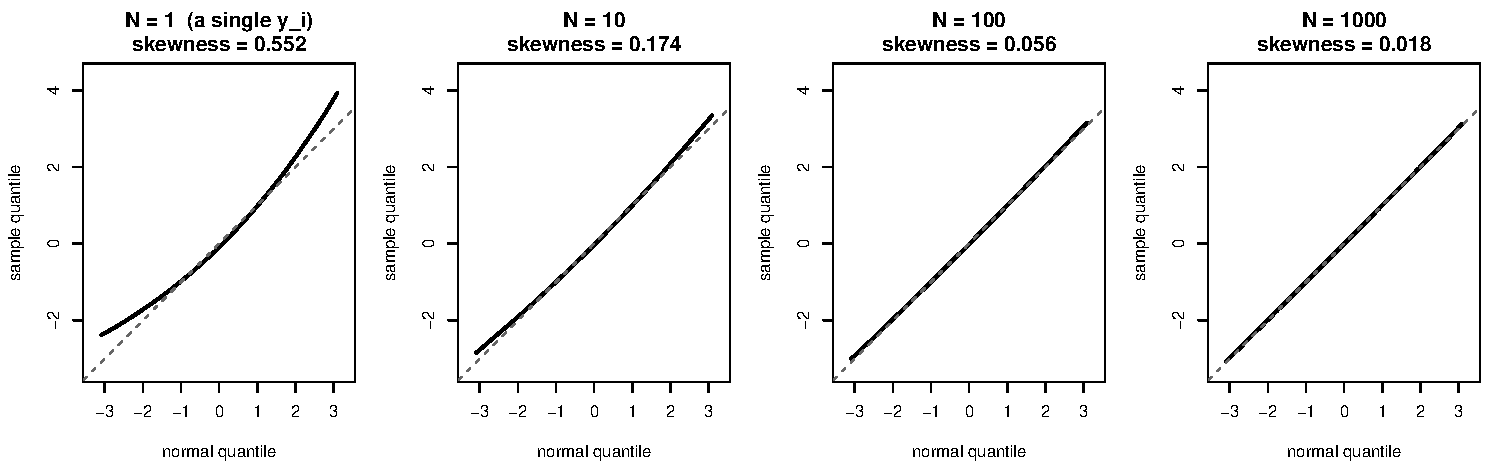
\includegraphics[width=\textwidth]{figures/q5_sampling_distributions.pdf}
\caption{Simulated distribution of $\bar{y}_N$ at $N = 10$, $100$ and $1000$,
each standardised to mean zero and unit variance so that only shape is
compared, with the standard normal density overlaid.}
\label{fig:q5}
\end{figure}

\emph{A note on the number of replications.} The lab notes use $M = 1000$,
which is ample for a variance, but part (4) estimates a \emph{third} moment and
that is far noisier. The standard error of a sample skewness is approximately
$\sqrt{6/M}$, so $M = 1000$ would give about $0.078$ --- more than four times
the value being measured at $N = 1000$, and the pattern would be buried in
noise. Raising $M$ to $500{,}000$ brings that standard error down to $0.0035$,
which is what makes the comparison in Table~\ref{tab:q5-skew} meaningful.

%==============================================================================
\appendix
\section{Complete R script}
\label{app:code}
%==============================================================================

The listing is read directly from the \code{.R} file at compile time, so it is
a verbatim copy of the code that produced the results above.

\subsection{\texorpdfstring{\code{R/q5\_simulation\_asymptotics.R}}{R/q5\_simulation\_asymptotics.R}}
\lstinputlisting[style=Rcode,caption={\code{R/q5\_simulation\_asymptotics.R}
--- Q5, simulation and asymptotics.},label={lst:app-q5}]%
{R/q5_simulation_asymptotics.R}

\end{document}
